

\section{Polar Coordinates \& Hyperbolic Functions}

\subsection{Polar Coordinates}
\begin{center}
    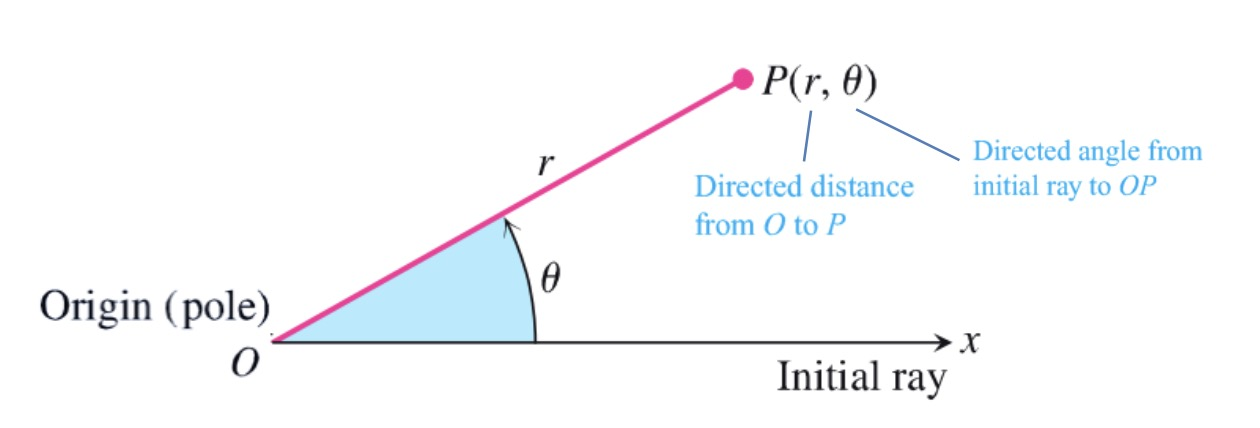
\includegraphics[width=0.6\textwidth]{./img/polar.jpg}

\end{center}
\begin{definition}
    {Equations relating Rolar and Cartesian coordinates}
    We can convert a Cartesian equation to polar equation using:
    \[x=r\cos\theta,\quad y=r\sin\theta\]
    We can also see that:
    \[r^2=x^2+y^2.\quad \tan\theta=\frac{y}{x}\]
    The polar equation for the circle $r^2 = x^2 + y^2$ is simply $r=a$.
\end{definition}
% \begin{knBox}
%     {Polar equations of ellipse}
%     In Cartesian form, an ellipse can be expressed as:
%     \[\frac{(x+c)^2}{a^2}+\frac{y^2}{b^2}=1,\quad\text{where }c=\sqrt{a^2+b^2}\]
%     Then we can write in polar form:
%     \[r=\frac{a(1-e^2)}{1+e\cos\theta},\quad\text{where }e=\frac{\sqrt{a^2+b^2}}{a}\]
% \end{knBox}
% \begin{theorem}
%     {Slope of polar curves}
%     The slope of a polar curve at a point is given by:
%     \[\frac{dy}{dx}=\frac{r\cos\theta+r'\sin\theta}{-r\sin\theta+r'\cos\theta}\]
%     \tcblower
%     To the the slope of the tangent to the unit circle at Cartesian coordinates $(\frac{1}{2},\frac{\sqrt{3}}{2})$:

%     We can find the the polar coordinates to be $(1,\frac{\pi}{3})$ using $\cos^{-1}\frac{1}{2}=\frac{\pi}{3}$, then we can use the formula to find the slope:
%     \[\frac{dy}{dx}=\frac{1\cos\frac{\pi}{3}+1'\sin\frac{\pi}{3}}{-1\sin\frac{\pi}{3}+1'\cos\frac{\pi}{3}}=-\frac{1}{\sqrt{3}}\]
% \end{theorem}
\begin{knBox}
    {Graphing}
    We can easily graph any polar formula $r=f(\theta)$ following the following steps:
    \begin{enumerate}
        \item Plot $r\ -\ \theta$ graph. If the function involves trigo functions, we can simply translate its graph. The height at a certain point is the distance from the origin.
        \item Then we can simply trace the graph from the left, and plot the points according to the distance from the origin at each angle. Using the eqations above, we can also find the Cartesian coordinates.
        \item If the graph is symmetric, we can simply copy the other half.
    \end{enumerate}
\end{knBox}

\subsection{Hyperbolic Functions}
\begin{definition}
    {Hyperbolic functions}
    Hyperbolic functions are defined as:
    \[\sinh x=\frac{e^x-e^{-x}}{2},\quad\cosh x=\frac{e^x+e^{-x}}{2}\]
\end{definition}
\begin{knBox}
    {Hyperbolic identities}
    The following identities hold for hyperbolic functions:
    \begin{enumerate}
        \item $\cosh^2x-\sinh^2x=1$
        \item $\cosh 2x=\cosh^2x+\sinh^2x$
        \item $\sinh 2x=2\sinh x\cosh x$
    \end{enumerate}
\end{knBox}
\begin{knBox}
    {Derivatives of hyperbolic functions}
    The derivatives of hyperbolic functions are:
    \begin{enumerate}
        \item $\frac{d}{dx}\sinh x=\cosh x$
        \item $\frac{d}{dx}\cosh x=\sinh x$
        \item $\frac{d}{dx}\sinh^{-1}x=\frac{1}{\sqrt{x^2+1}}$
        \item $\frac{d}{dx}\cosh^{-1}x=\frac{1}{\sqrt{x^2-1}}$
    \end{enumerate}
\end{knBox}